\chapter[Implementación]{
  \label{chp:implementacion}
  Implementación
}
\minitoc
\newpage

Neste capítulo comentarase a implementación daquelas partes do proxecto que merezan unha explicación máis detallada.

O código fonte pode atoparse no CD que se adxunta con esta memoria. Tamén está publicado de xeito íntegro en \textbf{GitHub} (Ver sección \ref{github}) no seguinte repositorio: \url{https://github.com/FerbLee/RSS-Radio}

\section{Estrutura xeral do código fonte}

Seguiuse a estrutura xenérica dos proxectos de Django que se amosa na figura \ref{fig:estrutura}. Creáronse dous paquetes: radio01 e rss\_feed, dos cales só se amosa expandido o primeiro. Para máis detalles do segundo, pódese ver a figura \ref{fig:project_tree} .

\begin{figure}[h]
	\centering
	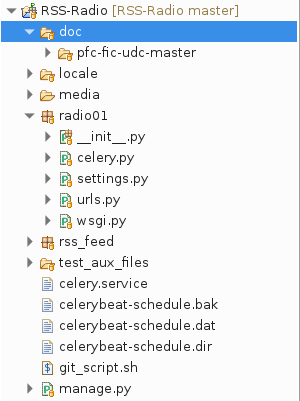
\includegraphics[scale=0.7,keepaspectratio=true]{./images/estrutura_impl.png}
	\caption{Estrutura do código fonte do proxecto.}
	\label{fig:estrutura}
\end{figure} 


A motivación destes dous paquetes é separar o código propio da aplicación, no de rss\_feed, e os ficheiros de configuración do servizo, no de radio01. Deste modo sería posible, de desexalo, crear novas aplicacións e poñelas a funcionar sobre o mesmo servidor sen necesidade de facer cambios nas que xa están a funcionar.

En radio01 atópanse os seguintes ficheiros: 

\begin{itemize}
	\item \textbf{settings.py:} Neste defínense, entre outras cousas, as aplicacións utilizadas por django (celery, django-bootstrap4...), os middlewares utilizados, os datos de conexión á base de datos e os subdirectorios que o sistema ha de coñecer. 

	\item \textbf{urls.py:} Relaciona cada aplicación coa súa URL. Nos paquetes de aplicación tamén hai un urls.py que define, dentro da aplicación, URL's relativas á definida no do paquete xeral. Neste proxecto, por exemplo, definiuse \textit{servername[:Porto]/rss\_feed} coma URL da aplicación, polo tanto, para acceder unha vista definida coma \say{vista1} de rss\_feed teríase que ir a \textit{servername[:Porto]/rss\_feed/vista1} 
	
	\item \textbf{celery.py:} Ficheiro de configuración de Celery.
	
	\item \textbf{wsgi.py:} Configuración da interface WSGI para aplicacións de Python (ver capítulo \ref{chp:tecnologia})
	
\end{itemize}

En rss\_feed atópanse os módulos propios da aplicación, incluíndo o código dos procesos periódicos do servidor dos que xa se falou en capítulos anteriores.


\section{Ficheiros de imaxe}

A diferenza dos ficheiros de audio, as imaxes amosadas si son gardadas en almacenamento propio. Serializar os ficheiros de imaxe para gardalos en base de datos non ofrece a penas vantaxes e sí incrementan o custo en almacenamento de xeito sensible, polo que se decidiu gardar os ficheiros nun directorio do servidor e, na base de datos, os seus metadatos e a ruta 
 ao ficheiro.
 
As imaxes son recollidas de dúas formas:

\begin{itemize}
\item \textbf{Subida manual:} Utilízase para os avatares de usuario e as imaxes da emisora.
\item \textbf{Descarga de un servidor externo:} Ao engadir un programa, as imaxes asociadas a eles e aos seus episodios descárganse do enlace que da o campo de imaxe de RSS (se existe). Dado que moitos servidores, por motivos de seguridade, bloquean as peticións de axentes descoñecidos, utilizáronse as cabeceiras de Firefox. Pode verse o código no listado \ref{lst:image}.
\end{itemize}

En calquera dos dous casos, as imaxes gárdanse no directorio \say{media}, agrupadas en subcarpetas por ano e mes. Nese mesmo directorio hai outra subcarpeta \say{default} onde se gardan as imaxes por defecto para aquelas entidades sen unha de seu.


\begin{lstlisting}[language=Python, caption=Código da función create\_image do módulo rss\_link\_parsers.py, label=lst:image]
def create_image(image_url):

	creation_date = timezone.now()
	original_image_name = os.path.basename(image_url)
	image_name = creation_date.strftime("%d%H%M%S") + '-' + original_image_name.lower()
	
	opener = urllib.request.build_opener()
	opener.addheaders = [('User-Agent','Mozilla/5.0')]
	urllib.request.install_opener(opener)
	image_file = urllib.request.urlretrieve(image_url)
	
	with open(image_file[0],'rb') as ifd: 
	
	new_image_instance = Image()
	new_image_instance.path.save( image_name, File(ifd) )
	
	new_image_instance.creation_date = creation_date
	new_image_instance.name = original_image_name
	new_image_instance.alt_text = original_image_name.lower()
	new_image_instance.original_url = image_url
	
	new_image_instance.save()
	
	return new_image_instance
\end{lstlisting}



\section{A vista de engadir programa}

Como se mencionou no capítulo \ref{chp:disenho}, empregouse un patrón \textbf{estratexia} para o deseño dos lectores de RSS. Implementouse, para isto, unha superclase \textbf{\textit{RSSLinkParser}} cun método \textit{parse\_and\_save} que crea os novos programas e episodios. Ese método apóiase en dous auxiliares que serán implementados polas súas clases fillas: 

\begin{itemize}
	\item \textbf{parse\_program:} Identifica os campos do programa do RSS e devolve un obxecto Program.
	\item \textbf{parse\_episode:} Identifica os campos de episodio e devolve un obxecto Episode. Execútase unha vez por elemento na lista de de episodios do RSS.
\end{itemize}

Ningún dos dous métodos crea entradas novas na base de datos, iso corre da conta da superclase.

Desta forma, basta con instanciar o tipo de \textit{RSSLinkParser} axeitado antes de aplicar o método de creación dos obxectos. A decisión de qué subclase utilizar, tómase na función \textit{add\_content} do módulo views.py en base a palabras clave contidas no enlace RSS introducido polo usuario (ver formulario de creación de programa na figura \ref{fig:add_program}).De non atopar ningunha delas, probará con todos os parsers existentes ata atopar o primeiro que non levante unha excepción. 

Se ningún parser da interpretado o RSS, o usuario será redirixido a unha páxina de erro.

\begin{figure}[h]
	\centering
	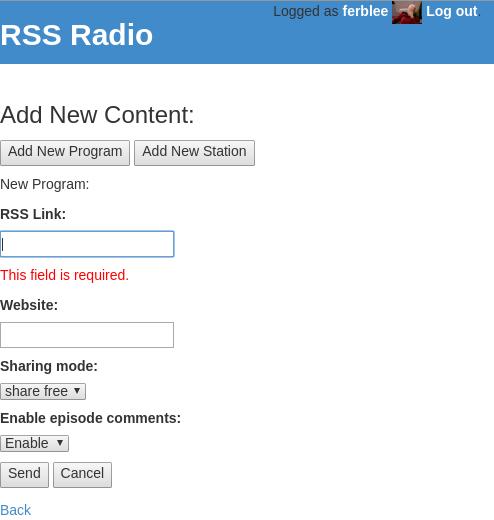
\includegraphics[scale=0.6,keepaspectratio=true]{./images/add_program_final.png}
	\caption{Formulario de engadir programa.}
	\label{fig:add_program}
\end{figure} 

\section{A tradución}

A tradución implementouse mediante as ferramentas que Django prové: \textit{i18n} para a tradución de texto estático dos templates e \textit{ugettext} para o texto xerado no código Python. Ambas válense do paquete gettext de GNU. 

O procedemento consiste elixir un idioma base e etiquetar aquelas cadeas de texto que sexan sensibles de seren traducidas. Unha vez estas estean marcadas, utilizaranse as ferramentas de Django para xerar un \textbf{ficheiro de extensión .po} por cada lingua que se queira habilitar. Estes ficheiros créanse no directorio marcado no ficheiro de settings.py, no caso deste proxecto, a carpeta \say{locale} que se ve na figura \ref{fig:estrutura}.

Os arquivos .po son ficheiros de texto que relacionan as cadeas de texto no idioma de base coa súa tradución no idioma elixido. Móstrase un exemplo na figura \ref{fig:traducion}. Neste proxecto elixiuse o Inglés coma lingua base e escribiuse unha tradución ao Galego.

\begin{figure}[h]
	\centering
	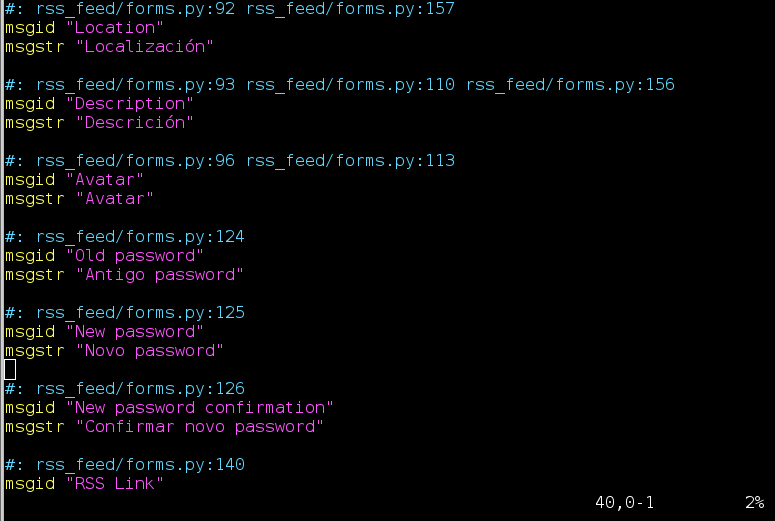
\includegraphics[scale=0.5,keepaspectratio=true]{./images/traducion.png}
	\caption{Fragmento do ficheiro .po para a tradución ao Galego.}
	\label{fig:traducion}
\end{figure} 


\section{O contador de escoitas}

Implementouse un contador das escoitas de cada capítulo. Cando un usuario comeza a reproducir o ficheiro de audio, mándase unha petición asíncrona ao servidor mediante \textbf{Ajax} para incrementar en 1 as escoitas do episodio na base de datos. Ese dato non é refrescado na interface automaticamente para non facer este proceso excesivamente transparente ao usuario.

Ao realizar esta acción, engádese o identificador do episodio a unha lista que se mantén nos \textbf{datos da sesión}, xa sexa un usuario identificado ou anónimo, de forma que nunha única sesión non se poida incrementar en máis de 1 as escoitas a un mesmo episodio. 

Isto faise para evitar, na medida do posible, as escoitas fraudulentas xa que este valor é un parámetro para o cálculo da popularidade.

 

\section{O panel de xestión}

O panel de xestión de emisora e programa comparten gran parte do código, así que poremos o primeiro coma exemplo dos dous. O panel de xestión componse de 4 vistas: 

\begin{itemize}
	\item \textbf{Edición de perfil:} Para cambiar o logo da emisora, o nome, a localización...
	
	\item \textbf{Xestión da emisión:} Mostrada na figura \ref{fig:panel}. É na que se dan de alta/baixa os programas a emitir ou se cambia o seu horario.
	
	\item \textbf{Administración:} Só visible a administradores de nivel \say{propietario}. Serve para dar de alta/baixa os administradores ou se cambian os seus permisos.
	
	\item \textbf{Borrado:}  Só visible a administradores de nivel \say{propietario}. Serve para borrar a emisora, para o que se require unha confirmación previa.
	
\end{itemize}

Para o caso da xestión de emisión atopámonos co problema de como darlle ao usuario unha ferramenta para seleccionar calquera programa existente na base de datos, pois pode ser unha lista moi extensa. Solucionouse isto aplicando unha ferramenta de selección de jQuery consistente nunha lista despregable que permite a busca por texto sobre a lista de opcións coa que sexa cargada (ver figura \ref{fig:panel}). 

Unha solución semellante se aplicou na vista de administración, pois a lista de usuarios a seleccionar tamén pode ser moi longa.

\begin{figure}[h]
	\centering
	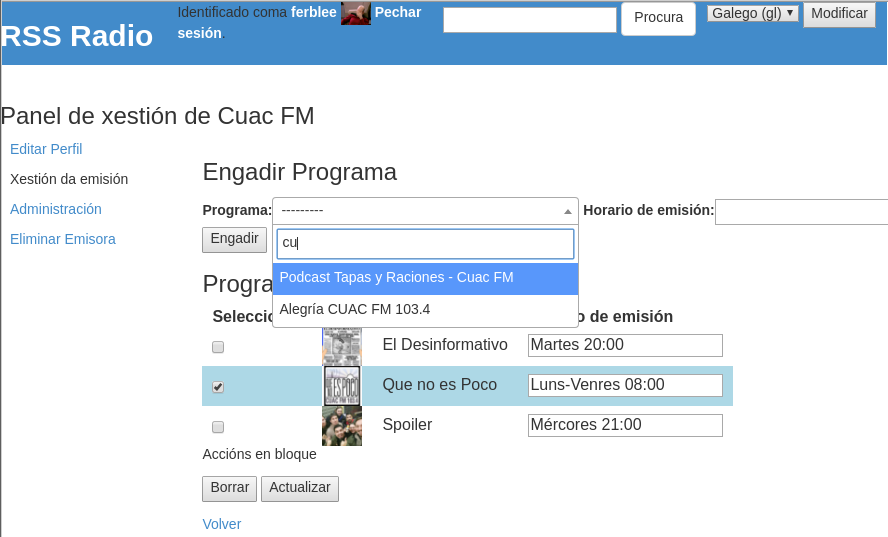
\includegraphics[scale=0.5,keepaspectratio=true]{./images/impl-panel.png}
	\caption{Panel de xestión dunha emisora. Vista de xestión da emisión. }
	\label{fig:panel}
\end{figure} 


\section{Execución dos procesos en Celery}

Para correr procesos de actualización sobre Celery, declaráronse os \say{endpoints} deses procesos no ficheiro celery\_endpoints.py do paquete rss\_feed. Os endpoints chámanse \textit{update\_rss \_info\_daemon}, para o proceso de actualización de episodios e \textit{update\_popularity \_rating\_daemon} para o do cálculo da popularidade. 

Eses endpoints serán utilizados polo worker de Celery para identificar os procesos e para poder configurar a súa periodicidade na sección de Celery do panel de administración de Django, como se ve na figura \ref{fig:celery}.

\begin{figure}[h]
	\centering
	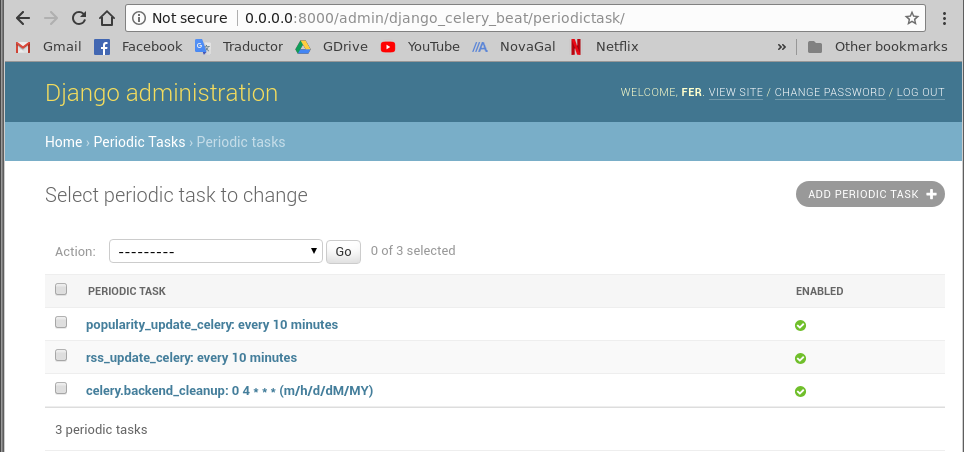
\includegraphics[scale=0.45,keepaspectratio=true]{./images/celery.png}
	\caption{Páxina de administración da aplicación, sección de procesos de Celery.}
	\label{fig:celery}
\end{figure} 


\section{Adaptabilidade a dispositivos móbiles}

Utilizouse a regra de CSS \textbf{@media} para definir diferentes estilos dependendo do tamaño da pantalla na que se amose o portal web. O listado \ref{lst:responsive} amosa o código para que un CSS-grid de 4 columnas pase a ser de 2 se a pantalla do dispositivo ten menos de 700 píxeles de ancho. 

\begin{lstlisting}[caption=Extracto da folla de estilos de index.html, label=lst:responsive]
@media only screen and (min-width: 700px) {

	.grid-item{
		border: 1px solid rgba(0, 0, 0, 0.8);
		text-align: center;
		padding: 20px;
	}
	.grid-container{
		display: grid;
		grid-template-columns: [col1-start]1fr [col2-start]1fr [col3-start]1fr [col4-start]1fr ;
		grid-gap: 20px;
	}
}

@media only screen and (max-width: 700px) {

	.grid-item{
		border: 1px solid rgba(0, 0, 0, 0.8);
		text-align: center;
		padding: 5px;
	}
	.grid-container{
		display: grid;
		grid-template-columns: [col1-start]1fr [col2-start]1fr;
		grid-gap: 2px;
	}
}
\end{lstlisting}
